\documentclass[12pt, a4paper]{report}
%\documentclass[11pt, a4paper]{article}

%====================== PACKAGES ======================
\usepackage[french]{babel}

\frenchbsetup{StandardLists=true}
\usepackage{enumitem}
\usepackage{pifont}

\usepackage[utf8x]{inputenc}
%\usepackage[latin1]{inputenc}

%pour gérer les positionnement d'images
\usepackage{float}
\usepackage{amsmath}
\usepackage{amsfonts}
\DeclareMathOperator{\dt}{dt}
\usepackage{graphicx}
%\usepackage{tabularx}
\usepackage[colorinlistoftodos]{todonotes}
\usepackage{url}

%pour les informations sur un document compilé en PDF et les liens externes / internes
\usepackage[pdfborder=0]{hyperref}
\hypersetup{
	colorlinks = true
	}

%pour la mise en page des tableaux
\usepackage{array}
\usepackage{tabularx}
\usepackage{multirow}
\usepackage{multicol}
\setlength{\columnsep}{50pt}

%pour utiliser \floatbarrier
%\usepackage{placeins}
%\usepackage{floatrow}

%espacement entre les lignes
\usepackage{setspace}

%modifier la mise en page de l'abstract
\usepackage{abstract}

%police et mise en page (marges) du document
\usepackage[T1]{fontenc}
\usepackage[top=2cm, bottom=2cm, left=2cm, right=2cm]{geometry}

%Pour les galerie d'images
\usepackage{subfig}

\usepackage{pdfpages}

\usepackage{tikz}
\usetikzlibrary{trees}
\usetikzlibrary{decorations.pathmorphing}
\usetikzlibrary{decorations.markings}
\usetikzlibrary{decorations.pathreplacing,calligraphy}
%\usetikzlibrary{decorations}
\usetikzlibrary{angles, quotes}
\usepackage{verbatim}

\usepackage{appendix}

\usepackage{comment}

\usepackage{xcolor}

%\PreviewEnvironment{tikzpicture}
%\setlength\PreviewBorder{0pt}%

%====================== INFORMATION ET REGLES ======================

%rajouter les numérotation pour les \paragraphe et \subparagraphe
\setcounter{secnumdepth}{4}
\setcounter{tocdepth}{4}

\hypersetup{							% Information sur le document
pdfauthor = {Stephan Runigo},			% Auteurs
pdftitle = {Documentation},			% Titre du document
pdfsubject = {Documentation},		% Sujet
pdfkeywords = {Document},	% Mots-clefs
pdfstartview={FitH}}	% ajuste la page à la largeur de l'écran
%pdfcreator = {MikTeX},% Logiciel qui a crée le document
%pdfproducer = {} % Société avec produit le logiciel

%======================== DEFINITION COMMANDES ========================
\newcommand{\si}[1]{\textsf{\textit {#1}}}
\newcommand{\mc}[1]{\mathcal{#1}}
\newcommand{\so}{\vspace{.323cm}}
\newcommand{\ib}[1]{\item {\bf #1}}
\newcommand{\fsb}[1]{\textsf{\textbf {\footnotesize #1}}}
\newcommand{\bi}[1]{\textbf{\textit {#1}}}
%======================== DEFINITION COMMANDES ========================
\newcommand{\mt}[1]{\text{#1}}
\newcommand{\pt}[1]{\dot{\text{#1}}}
%======================== DEBUT DU DOCUMENT ========================
%
\begin{document}
%
%régler l'espacement entre les lignes
\newcommand{\HRule}{\rule{\linewidth}{0.5mm}}
%
% Titre, résumé, ... %
%%
\begin{titlepage}
%
~\\[1cm]

\begin{center}
%\includegraphics[scale=0.5]{./presentation/chambreABulle}
\end{center}

\textsc{\Large }\\[0.5cm]

% Title \\[0.4cm]
\HRule

\begin{center}
{\huge \bfseries  La causalité\\
%titre 2\\[0.4cm]
 }
\end{center}

\HRule \\[1.5cm]

\begin{center}
%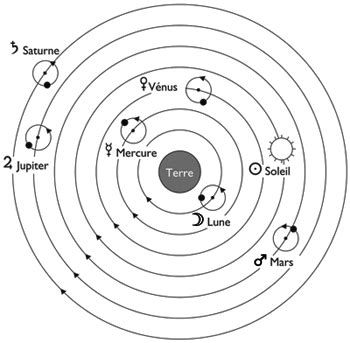
\includegraphics[scale=0.3]{./presentation/ptoleme}
\end{center}

\begin{center}
%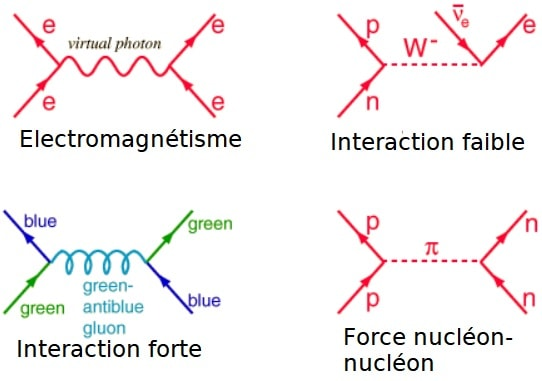
\includegraphics[scale=0.3]{./presentation/diagrammesInteractions}
\end{center}


% Author and supervisor
\begin{minipage}{0.4\textwidth}
\begin{flushleft} \large
%\emph{Auteur:}\\
%Stephan \textsc{Runigo}
\end{flushleft}
\end{minipage}
\begin{minipage}{0.4\textwidth}
\begin{flushright} \large
\emph{Auteur:}\\
Stephan \textsc{Runigo}
\end{flushright}
\end{minipage}

\vfill

% Bottom of the page
{\large \today}

\end{titlepage}

\newpage
\begin{center}
\Large
Résumé
\normalsize
\end{center}
\vspace{3cm}
\begin{itemize}[leftmargin=1cm, label=\ding{32}, itemsep=21pt]
\item {\bf Objet : } Souvenir des questions posés.
\item {\bf Contenu : } Définition, analyse, reflexion.
\item {\bf Public concerné : } Interressé à la question de l'âme.
\end{itemize}

\vspace{3cm}



\vspace{3cm}


%

%
% Table des matières
\tableofcontents
\thispagestyle{empty}
\setcounter{page}{0}
%
%espacement entre les lignes des tableaux
\renewcommand{\arraystretch}{1.5}
%
%====================== INCLUSION DES CHAPITRES ======================
%
~
\thispagestyle{empty}
%recommencer la numérotation des pages à "1"
\setcounter{page}{0}
\newpage
%\chapter{Formulaire}
\subsection{Mécanique analytique}

Action S et lagrangien L

Principe

\[
S = \int_{t_1}^{t_2} L(q_i, \dot{q}_i, t)dt \ \ \ \ \ \ \text{est extrémale}
\]

L'invariance du lagrangien par translation temporelle entraine le théorème :

\[
E \ \text{est une constante du mouvement}
\]

\subsection{Thermodynamique}

Énergie U, entropie S, température T, chaleur Q, travail W,  pression P, volume V

Principes
\[
dU = \delta Q + \delta W \ \ \ \ \ \ dS = \frac{\delta Q}{T}
\]
Théorème TdS
\[
dU = TdS - pdV
\]

\subsection{Quantique}
L'énergie est une observable, dans un système isolé,
\[
\mc{H}|\psi(x,t)\rangle=E|\psi(x,t)\rangle
\]


\[
\mc{H} = -i\hbar\frac{\partial}{\partial t} \ \ \ \ \ \ \ \mc{P} = i\hbar\frac{\partial}{\partial x}
\]

\chapter{Introduction}
\section{Définitions}
\subsection{}
On peut distinguer un sens commun et un sens scientifique au mot énergie (sens I et II).
%Chacun de ces deux sens peuvent être distingués

\begin{enumerate}[leftmargin=3cm, label=\Roman*{\bf .}]
\item {\bf Sens commun}
  \begin{enumerate}[label=\arabic*{\bf .}]
  \item Sens {\bf courant} : force, vigueur, vivacité (éthymologie : force en action)
  \item Sens {\bf spiritualiste} : principe, substance.
  \end{enumerate}
\item {\bf Sens scientifique}
  \begin{enumerate}[label=\arabic*{\bf .}]
  \item Sens {\bf économique} : source d'énergie exploitable économiquement (pétrole, charbon, gaz, éolien, hydrolique, solaire)
  \item Sens {\bf physique} : grandeur conservée lors d'une transformation d'un système isolé.
  \end{enumerate}
\end{enumerate}

\subsection{Sens économique}
Le pétrole, le charbon, le gaz sont des sources d'énergie dont le transport est un enjeux économique. Ainsi, il existe des pétroliers, des trains, des gazoducs qui les acheminent. On peut lire dans certains articles : {\it Le transport des énergies est un enjeux économique} (ne devrait-on pas dire "le transport du pétrole, du charbon et du gaz est un enjeux économique" ou "le transport des énergies fossiles est un enjeux économique" ?).

Également, on peut lire dans d'autres articles : {\it Le transport de l'énergie électrique est un enjeux économique}. On devrait plutôt dire "le transport de l'électricité est un enjeux économique".

\subsection{Sens physique}
La physique distingue le système et les grandeurs. En particulier, une onde électromagnétique est un système physique auquel on associe des grandeurs (longueur d'onde, amplitude, énergie). On peut alors lire dans certains article "une onde électromagnétique transporte de l'amplitude", ce qui est impropre, il faut plutôt dire "une onde électromagnétique possède une amplitude".

\subsection{Sens éthymologique}
Il faudrait préciser ce que l'on entend par "en action" : est-ce par opposition à "au repos" (il existerait des {\it forces en action} et des {\it forces au repos}), ou bien de façon plus philosophique par opposition à la puissance (il existerait des forces {\it en acte} et des forces {\it en puissance}). (en philosophie, {\it puissance} signifie {\it possibilité, faculté}, en physique, la puissance est une {\it énergie par unité de temps}, c'est différent).

\subsection{Sens spiritualiste}
Dans certains discours, des énergies s'opposent :
\begin{itemize}[leftmargin=1cm, label=\ding{32}, itemsep=1pt]
\item Des énergies positives s'opposent à des énergies négatives.
\item Des énergies bénéfiques s'opposent à des énergies maléfiques.
\item Des énergies vibratoires s'opposeraient à des énergies non-vibratoires.
\item Des énergies immatérielles s'opposeraient à des énergies matérielles.
\end{itemize}
On peut reconnaître dans certains de ces discours des {\it jugements de valeurs}, un discours sur le {\it bien et le mal}.

Dans ces discours, le mot énergie peut alors être remplacé par d'autre mots (vibration, onde, longueur d'onde) sans changer le sens du discours :
\begin{itemize}[leftmargin=1cm, label=\ding{32}, itemsep=1pt]
\item Énergies positives $=$ ondes positives, bonnes vibrations...
\item Énergies négatives $=$ vibrations négatives, mauvaises ondes...
\item Énergies vibratoires $=$ vibrations énergétiques...
\item Énergies bénéfiques $=$ "bonne longueur d'onde" $=$ "bonne synchronisation".
\item Énergies immatérielles $=$ indéfinissable.
%\item Énergies matérielles $=$ .
\end{itemize}
%Au {\footnotesize XVII}$^\text{e}$, Newton énonce la loi de la gravitation  universelle, unifiant la mécanique celeste et la mécanique terrestre. 

%\chapter{Thermodynamique}

\section{Variables d'état}
L'état d'un système thermodynamique est décrit par des variables d'états. Ces variables peuvent être fonction les unes des autres. En générale, trois variables d'états indépendante sont suffisante pour déterminer complètement l'état du système, les autres variables étant fonction des trois premières.

{\bf Exemples : }
Énergie U, entropie S, température T,  pression P, volume V, enthalpie H, énergie libre F, enthalpie libre G...

Lorsqu'un système thermodynamique est à l'équilibre, ses variables d'états sont constantes au cours du temps.

\section{Principes}

Les trois principes de la thermodynamique permettent de déterminer l'état d'équilibre d'un système thermodynamique.

La variation élémentaire d'énergie interne est égale à la somme des quantités élémentaires de chaleur et de travail apporté au système par l'extérieur :
\[
\tag{1}dU = \delta Q + \delta W
\]

La variation élémentaire d'entropie est égale à la quantité élémentaire de chaleur apporté par l'extérieur divisé par la température :
\[
\tag{2}dS = \frac{\delta Q}{T}
\]

L'entropie s'annule si la température est nulle :
\[
\tag{3}S = 0 \mt{ si } T=0
\]

\section{Théorème}
\begin{minipage}[c]{.45\linewidth}
Des principes, on tire le théorème TdS :
\end{minipage}
\hfill
\begin{minipage}[c]{.45\linewidth}
\[
dU = TdS - pdV
\]
\end{minipage}

\section{Définitions}
On définie les fonctions suivantes :

L'énergie libre : 
\[
F=U-TS
\]

L'enthalpie :
\[
H=U-PV
\]

L'enthalpie libre :
\[
G = U-TS-PV
\]


\chapter{Electrodynamique}

\section{Un exercice pédagogique}
\subsection{Générateur et circuit électrique}
%\subsection{Effet joule}
\begin{minipage}[c]{.5\linewidth}
\hspace{0.7cm}Un générateur électrique G (pile électrochimique) maintient une tension électrique (ou force électromotrice) U entre ses bornes. Cette tension produit un courant électrique I dans le circuit électrique contenant des fils de résistance négligeable et le conducteur ohmique R.
\end{minipage}
\hfill
\begin{minipage}[c]{.5\linewidth}
\begin{center}
\begin{tikzpicture}
\draw [very thick] (0,0) node [above]{G} circle(0.7);
\draw [->, very thick] (1,1) -- (-1,1) node [above]{U};
\draw [thick] (-1,3) -- (-2,3) -- (-2,0) -- (2,0) -- (2,3) -- (1,3);
\draw [very thick] (-1,3.3) -- (-1,2.7) -- (1,2.7) -- (1,3.3) -- cycle;
\draw (0,3) node {R};
\draw [very thick] (2.3,1.7) node [below right]{I} -- (2,1.4) -- (1.7,1.7);
\end{tikzpicture}
\end{center}
\end{minipage}\vspace{0.5cm}

L'expérience montre que la température du conducteur ohmique s'élève, c'est l'effet Joule. Nous nous interressons aux transferts d'énergie responsable de cet échauffement :

Dans le générateur, de l'énergie électrochimique est convertie en énergie électrique, dans le conducteur ohmique de l'énergie électrique est convertie en énergie thermique. Nous souhaitons interpréter et évaluer cette dernière conversion.

Le conducteur ohmique R est cylindrique (longueur {\it l}, section {\it s}). La tension U est maintenue entre ses extrémités, il est parcouru par le courant I (le courant I est proportionnel à la tension U. C'est la loi d'Ohm : U $=$ R.I).

\begin{center}
\begin{tikzpicture}
\draw[thick] (0,0) ellipse (0.3cm and 0.7cm);
\draw (0,0.7) -- (10,0.7);
\draw (0,-0.7) -- (10,-0.7);
\draw [thick,->] (10,-1.4) -- (0,-1.4) node [left] {U};
\fill (5,0) -- (4.3,0.7) -- (4.7,0) -- (4.3,-0.7) -- cycle node [right] {I};
\draw (10,0.7) .. controls (10.5,0.7) and (10.5,-0.7) .. (10,-0.7);
\end{tikzpicture}
\end{center}

La tension U est une différence de potentiel entre les extrémité du conducteur ohmique, relié par définition au champ électrique {\bf E}

\subsection{Électrons libres et champ électrique}
Au niveau microscopique, le conducteur ohmique est constitué par un réseau d'ions positifs fixes
\begin{tikzpicture}
\draw (0,0) node [color=red] {$+$};\draw (0,0) [thick, color=gray!40] circle (0.3);
\end{tikzpicture}
et d'électrons mobile
\begin{tikzpicture}
\draw (0,0) node [color=blue] {$e^-$};
\end{tikzpicture}. L'ensemble étant électriquement neutre.
\begin{center}
\begin{tikzpicture}
\foreach \x in {-2,-0.5,...,3}
{\foreach \y in {1,2.5,...,11}
{\draw (\y,\x) node [color=red] {$+$};\draw (\y,\x) [thick, color=gray!40] circle (0.3);
%\draw (\y+0.75+0.3*rand,\x+0.75+0.3*rand) node {$e^-$};}}
\draw (\y+0.75*rand,\x+0.75*rand) node [color=blue] {$e^-$};}}
\draw [->, very thick] (4,0.25) -- (7,0.25) node [right] {{\bf E}};
\end{tikzpicture}
\end{center}
Le courant électrique est due au mouvement d'ensemble des électrons mobiles (libres) sous l'effet du champ électrique {\bf E} ( relié par définition à la tension U
% : {\bf E} $=-\frac{\partial}{\partial\mt{x}}$V(x)$\hat{\mt{x}}$
).

Soumis à une force de la part du champ électrique, les électrons libres sont mis en mouvement. Ils subissent alors des collisions avec les ions immobile, leurs cédant une partie de leur énergie cinétique. Les ions du réseau acquièrent alors de l'énergie de vibration, se traduisant par un échauffement du conducteur.

\subsection{Champ magnétique et vecteur de Poynting}

Le courant I produit un champ magnétique : Les lignes de champs sont des cercles, centré sur l'axe du conducteur, le champ est perpendiculaire à cet axe.




\chapter{Vocabulaire}
%Lorsque des scientifiques découvrent quelque chose de nouveau, ils le nomment. Le nom choisi peut être un nom propre, hommage ou clin d'œuil au découvreur ou à l'un des précursseur à 

\section{Larousse éthymologique}
{\bf Énergie }{\footnotesize XV}$^\text{e}$ s. {\it Jardin de santé}, du bas latin {\it energia} (saint Jérôme), emprunté au grec {\it energeia}, force en action. || {\bf énergique} fin {\footnotesize XVI}$^\text{e}$ s. || {\bf énergétique} 1768, {\it Encycl.}, « qui paraît avoir une énergie innée »; sens actuel, fin {\footnotesize XIX}$^\text{e}$ s. (1909, L. M.); du grec {\it energetikos}.

{\bf Force} 1080, {\it Roland}, du bas latin {\it fortia}, pl. neutre subst. de {\it fortis}, courageux puis fort. || {\bf forcer} {\footnotesize XIII}$^\text{e}$ s. {\it Chr d'Antioche}, du lat. pop. {\it fortiare}, de {\it fortia}. [...]% || {\it forçage} {\footnotesize XII}$^\text{e}$ s.


\section{Vocabulaire de la philosophie}
{\bf Force} — \si{Vulg.} {\bf 1.} (Souvent opp. {\it droit}$^1$). Contrainte :
« Céder à la force ». — {\bf 2.} Puissance d'action : « Les forces morales ».
{\it Idée-force} (Fouillée) : la représentation$^1$ considérée comme poussant
à l’action$^2$. — {\bf 3.} Agent$^1$ physique : « Les forces naturelles ».

— \si{Math.} {\bf 4.} En mécanique : tout ce qui est capable de modifier l’état de
repos ou de mouvement d’un corps (cf. {\it Inertie}$^{\,2}$). — {\bf 5.}
{\it Force vive} (syn. : énergie actuelle) : demi-produit de la masse par le
carré de la vitesse (1/2 mv$^2$).

— \si{Méta.} {\bf 6.} L’énergie*, considérée comme le principe indéfinissable
qui produit les phénomènes de l’univers : « Force et matière » (Büchner) ;
« La persistance de la force » (Spencer). — {\bf 7.} {\it Chez Leibniz} :
voir {\it Substance}$^1$.

{\bf Énergétique} — \si{Phys.} {\bf 1.} Science des
propriétés générales de l’énergie$^1$,
abstraction faite des caractères$^2$
particuliers propres à chacune des
formes sous lesquelles elle apparaît.
— {\bf 2.} Théorie physique fondée sur
le principe de la conservation* de
l'énergie et sur le principe de moindre
action* : « Le système$^2$ énergétique
a pris naissance à la suite de la
découverte du principe
de la conservation de l'énergie. C’est
Helmholtz qui lui a donné sa forme
définitive » (H. Poincaré).

{\bf Énergétisme} — \si{Méta.} \fsb{S. norma.} La théorie
énergétique$^2$ érigée en système métaphysique qui fait de l'{\it énergie}
la substance même du monde : « L’énergétisme d'Ostwald ».
% 66

{\bf Énergie} — \si{Phys.} L'{\it énergie} d'un système de corps se mesure
par le travail$^1$ mécanique qu’il est capable
de produire. {\it Énergie actuelle} ou
{\it cinétique} : celle qui se manifeste par
le mouvement (égale à la somme
des forces$^5$ vives du système).
{\it Énergie potentielle} : celle qui n'existe
qu’en puissance, {\it i. e.} travail que les
forces intérieures du système effectueraient si les corps qui le composent obéissaient à l'action de ces
forces.


%
%\chapter{Formulaire}
\subsection{Mécanique analytique}

Action S et lagrangien L

Principe

\[
S = \int_{t_1}^{t_2} L(q_i, \dot{q}_i, t)dt \ \ \ \ \ \ \text{est extrémale}
\]

L'invariance du lagrangien par translation temporelle entraine le théorème :

\[
E \ \text{est une constante du mouvement}
\]

\subsection{Thermodynamique}

Énergie U, entropie S, température T, chaleur Q, travail W,  pression P, volume V

Principes
\[
dU = \delta Q + \delta W \ \ \ \ \ \ dS = \frac{\delta Q}{T}
\]
Théorème TdS
\[
dU = TdS - pdV
\]

\subsection{Quantique}
L'énergie est une observable, dans un système isolé,
\[
\mc{H}|\psi(x,t)\rangle=E|\psi(x,t)\rangle
\]


\[
\mc{H} = -i\hbar\frac{\partial}{\partial t} \ \ \ \ \ \ \ \mc{P} = i\hbar\frac{\partial}{\partial x}
\]

%
%
\begin{appendix}
%

%%%%%%%%%%%%%%%%%%%%%
\chapter{Glossaire}
%%%%%%%%%%%%%%%%%%%%%

\begin{itemize}[leftmargin=1cm, label=\ding{32}, itemsep=2pt]
\item {\bf application} : en mathématique, synonyme de fonction.
\item {\bf } :
\item {\bf } :
\item {\bf quanton} : particule élémentaire satisfaisant à l'équation de schrödinger.
\item {\bf } :
\item {\bf } :
\item {\bf } :
\end{itemize}


%%%%%%%%%%%%%%%%%%%%%%%%%%%%%%%%%%%%%%%%%%%%%%%%%%%%%%%%%%%%%%%%%%%%%%%%%%%%%%%%%%%%%

%

%%%%%%%%%%%%%%%%%%%%%
\chapter{Espace vectoriel}
%%%%%%%%%%%%%%%%%%%%%

%%%%%%%%%%%%%%%%%%%%%%%%%
\section{Ensemble et application}
%%%%%%%%%%%%%%%%%%%%%%%%%
%$\mathcal{}$
Un ensemble est une collection d'objets. Ces objets sont appelés éléments (a) de l'ensemble ($\mathcal{A}$) :
\[
 a \in \mathcal{A}
\]


Une application ($f$) met en relation chaque élément ($a$) d'un ensemble ($\mathcal{A}$, dit de départ) avec un élément ($b$) d'un autre ensemble ($\mathcal{B}$, dit d'arrivé) :
\begin{align*}
f :\ \ \ \ \ \ \ \ \ \mathcal{A} \ \  & \rightarrow \ \ \ \mathcal{B} \\
a \ \ & \mapsto \ \ b = f(a)
\end{align*}

Une loi de composition est une application qui associe deux éléments (éventuellement du même ensemble) à un troisième élément. 
\begin{align*}
f :\ \ \ \ \ \ \ \ \ \mathcal{A} \times \mathcal{B} \ \  & \rightarrow \ \ \ \mathcal{C} \\
(a,b) \ \ & \mapsto \ \ c = f(a,b)
\end{align*}

Une loi de composition est dite interne si $\mathcal{A} = \mathcal{B} = \mathcal{C}$, externe sinon.



%%%%%%%%%%%%%%%%%%%%%%%%%
\section{Espace vectoriel}
%%%%%%%%%%%%%%%%%%%%%%%%%
%
Un espace vectoriel est un ensemble (ses éléments sont appelés vecteur), possédant une loi de composition interne (la somme de deux vecteurs d'un espace vectoriel appartient à cet espace) et une loi de composition externe (la multiplication par un scalaire d'un vecteur d'un espace vectoriel appartient à cet espace).


%%%%%%%%%%%%%%%%%%%%%%%%%%%%%%%%%%%%%%%%%%%%%%%%%%%%%%%%%%%%%%%%%%%%%%%%%%%%%%%%%%%%%

%

%%%%%%%%%%%%%%%%%%%%%
\chapter{Transformation de fourier}
%%%%%%%%%%%%%%%%%%%%%

%%%%%%%%%%%%%%%%%%%%%%%%%
\section{Série de fourier}
%%%%%%%%%%%%%%%%%%%%%%%%%
%
Une fonction périodique (de période $T$) est égale à une somme discrète de sinusoïde :
\[
f_T(x)=a_0 + \sum_{n=1}^\infty \left( a_n \cos \frac{2 n \pi x}{T} + b_n \sin \frac{2 n \pi x}{T} \right)
\]
$a_n$ et $b_n$ sont les coefficient de fourier de $f_T(x)$.

%%%%%%%%%%%%%%%%%%%%%%%%%
\section{Transformé de fourier}
%%%%%%%%%%%%%%%%%%%%%%%%%
%
Une fonction quelconque est égale à une somme continue de sinusoïde :
\[
f(x) = \int_{-\infty}^\infty e^{2 i \pi \nu x}\widehat{f}(\nu) d\nu
\]
$\widehat{f}(\nu)$ est la transformé de fourier de $f(x)$.

%%%%%%%%%%%%%%%%%%%%%%%%%%%%%%%%%%%%%%%%%%%%%%%%%%%%%%%%%%%%%%%%%%%%%%%%%%%%%%%%%%%%%

%
%\newpage
%
\end{appendix}
%

%
%====================== INCLUSION DE LA BIBLIOGRAPHIE ======================
%
%récupérer les citation avec "/footnotemark" : 
\nocite{*}
%
% choix du style de la biblio
\bibliographystyle{plain}
%
% inclusion de la biblio
\cleardoublepage
\addcontentsline{toc}{chapter}{Bibliographie}
\bibliography{bibliographie.bib}
%
%====================== FIN DU DOCUMENT ======================
%
\end{document}
%%%%%%%%%%%%%%%%%%%%%%%%%%%%%%%%%%%%%%%%%%%%%%%%%%%%%%%%%%%%%%%%%%%%%%%%%%%%%%%%%
